\documentclass{article}

\usepackage[utf8]{inputenc}
\usepackage[T1]{fontenc}
\usepackage[francais]{babel}
\usepackage[top = 1.5cm, left = 1.5cm, right =1.5cm, bottom = 1.5cm]{geometry}
\usepackage[pdfborder ={0 0 0}]{hyperref}
\usepackage{graphicx}
\usepackage{xcolor}
\usepackage{multicol}
\usepackage{lscape}
\usepackage{datatool}
\usepackage{pdfpages}
\usepackage{rotating}
\usepackage{xspace}
\usepackage{titlesec}
\usepackage{colortbl}
\usepackage{roboto}

\definecolor{title-color}{gray}{0.30}
\definecolor{heading-color}{gray}{0.90}

\setlength{\parindent}{15pt}
\setlength{\parskip}{5pt}

\titleformat{\section}
  {\clearpage\normalfont\sffamily\Huge\bfseries\centering\robotoslab\color{title-color}}
  {}{0pt}{\bigskip}

\titleformat{\subsection}
  {\normalfont\sffamily\LARGE\bfseries\robotoslab\color{title-color}}
  {\thesubsection}{1em}{}

\titleformat{\subsubsection}
  {\normalfont\sffamily\large\bfseries\robotoslab\color{title-color}}
  {\thesubsubsection}{1em}{}

\begin{document}

\begin{titlepage}
\begin{figure}
\end{figure}

\title{\vspace{1cm}{\Huge \bf{\color{title-color}\robotoslab Management Project} } \\ \vspace{2cm} \bf{\color{title-color}\robotoslab Mold \& Co in China} \vspace{1cm} \\
}
\begin{figure}
\begin{center}
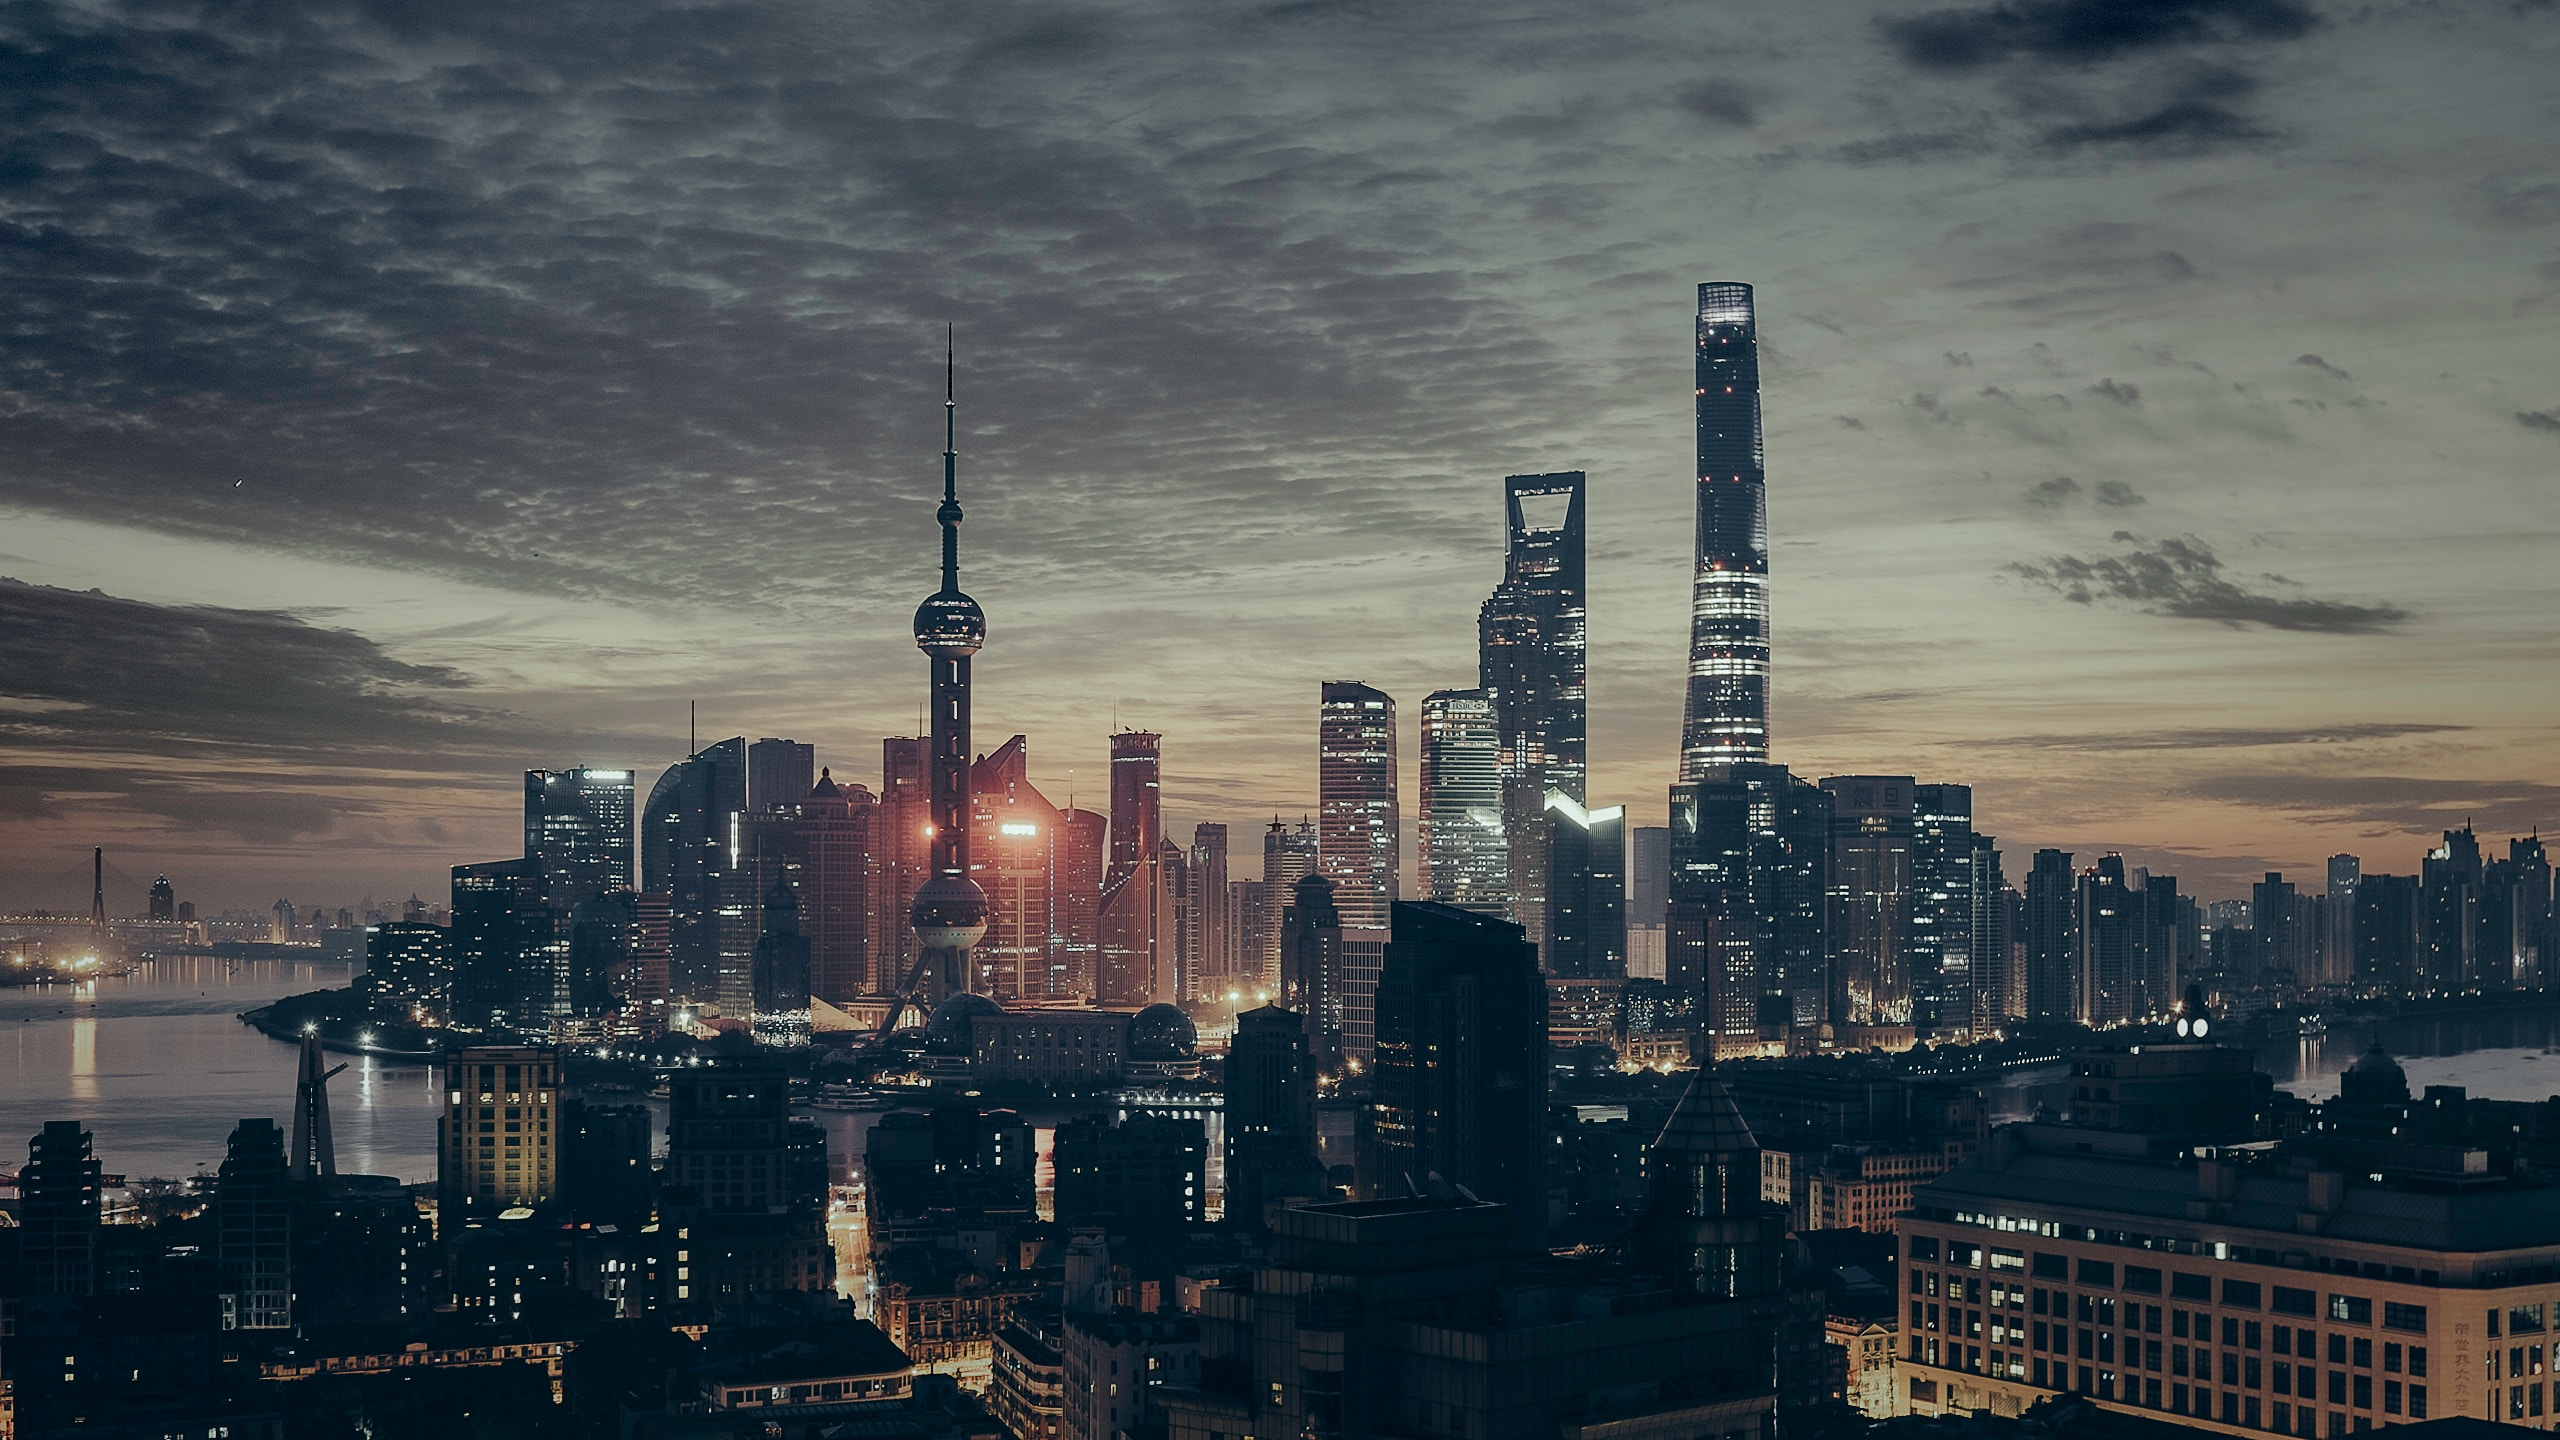
\includegraphics[scale = 0.2]{Img/china-illustration.jpg}
\end{center}
\end{figure}
\author{\Large{Marie \bsc{Chiaverini}} \Large{Baptiste  \bsc{Saclier}} \\\Large{Vadim  \bsc{Crochet}} \Large{Antoine  \bsc{Caillet}} \\\Large{Romain  \bsc{Junca}}}
\date{}
\vfill 
\end{titlepage}
\maketitle
\vspace{5.5cm}
\Large{CESI school of engineers} \hfill \Large{Tutor : Thierry \bsc{BLANC}}
\thispagestyle{empty}
\setcounter{page}{0}
\newpage

\renewcommand{\contentsname}{Table of contents}
\tableofcontents

\newpage
\renewcommand{\listfigurename}{List of figures}
\listoffigures

\newpage

\newcommand{\projectname}{ChineseTooth\xspace}
\newcommand{\companyname}{Cesi conseil\xspace}
\newcommand{\moldco}{MOLD \& Co.\xspace}

\section{Introduction}

This document describes all aspects of the \projectname project which the main goal is to install IT systems around the new production line in the eco-city of Taijin.
This project includes a social and ecological aspect in order to fit to the requirements of Taijin city guidelines.

In this document, we describe what are the goals, the processes, the planning and the risk of such deployment in China.

\section{Project description}

% Description précise de tout les aspects du projet
% Quel sont les objectifs ? 
% Dans quel contexte le projet évolue il ?
% Quels sont les contraintes (Environnement, Social, Temps, Législation) ?
% Quels sont les forces et les faiblesses ?

The main goal is to install a toothbrush production line in the eco-city of Taijin in China.
Our company is workig for \moldco to make this production line a reality.

Ou main guidelines in this project is to install a production line that can produce a great amount of toothbrushes within an eco-city.
This project needs to be respectful of the surrounding environnement and social aspects of the project's stakeholders.

\subsection{Specifications}

This project has to achieve the following specifications.

The production line must contains all the required machines to automate the production of toothbrushes.
Theses machines include moulting machine, stamping machine, tufting machine, bristle cutter machine, bristle trimming machine and Packaging machine.
These machines need to be bought and connected to each other in order to build the full product.

To connect all the machines in the assembly line, the project requires also a full digital connection to an internal network.
This network group all connected machines and database servers to store monitoring informations about the production.
These informations need to represent the current production, the past production and potential errors in the production line.

The production line is fully automated throw this network and the production is regulated to produce exactly what is needed.
This automatisation brings many advantages including the environmental impact reduction, reduction of the storage requirement of finished products and 24/7 production in case of huge demand.

The informations collected need to be displayed to the employees in charge of the production line.
These informations are displayed throught an interface reading the monitoring data from the database.
A master server has to be installed in order to control all machines and to control the production flow.

Several materials are required to produce toothbrushes.
These materials are plastic, nylon, brass wire, paper box packing, plastinc hard container packaging, high frequency blister packaging and Blister card packaging.
The project must include a storage space for all these material and human resources to load the resources in the appropriate machines.

All the production line machines, storage and digital network requires engineering the organise all these components depending on the space available and the shape of the building.
Enginieering human resources are required to create, configure and install manitoring system.
Human resources may also be required to manipulate machines, connect each machine to the other and install network.

\subsection{Forces}

The forces of the project are mainly focused on the high effeciency of the production line.
This high effeciency is garanteed by the monitoring system and the automatic management of the amount of product produced on the assembly line.
This project represents a great opportunity to modernize the production of \moldco and automate the assembly line.
By automating the assembly line, \moldco gain a lot of money on storage of manufatured products and human resources.

\subsection{Weaknesses}

This project have also small weakness that may have an impact on risks
(Risk managment will be covered in the section \ref{risk-management}).

The main weakness are the important amount of advanced technologies that requires a great amount of high qualified employees in charge of the installing and maintaining the autonomous system of the assembly line.
Another weakness is the requirement of heavy and pricy machines that can represent a major part of the project's costs.

\section{Actors and Stakeholders}

% Quels sont les différents acteurs ayant un impact sur le projet ?
% Quels sont les parties prenantes et leur position dans le projet ?
% Quels sont les équipes que l'on doit mettre en place ?

We have assembled all the actors of the project in a clear and precise way in order to identify them. You will first find the different actors who have an impact on the project. Secondly, the stakeholders and their position in the project. Finally, the teams that need to be set up.

\subsection{Actors impacting the project}

You will find below a table containing all the actors having an impact on the project. All the stakeholders were identified and analysed according to the client's needs by the \companyname team.

There are four columns :

\begin{description}
    \item[Name] : it is the name of the actor and stakeholder.
    \item[External or Internal to \moldco companie] : The actor in question is internal or external to \moldco. This is its positioning within the project.
    \item[State] : what type of domain is the actor affiliated.
    \item[Influence level] : this is the level of importance of the actor in the project.
\end{description} 

\begin{figure}[h]
\centering
\begin{tabular}{| p{4cm} | c | c | c |}
    \hline
    \rowcolor{heading-color}\multicolumn{1}{|c|}{Name} & External or internal & Status & Influence level \\
    \hline
    Mold and Co - HR department & Internal & Supervision & Important \\
    \hline
    Mold and Co - Production department & Internal & Manufacturation & Important \\
    \hline
    Mold and Co's direction & Internal & Client & Important \\
    \hline
    \companyname & External & Provider & Important \\
    \hline
    Mold and Co's - It department & Internal & Supervision & Medium \\
    \hline
    Mold and Co's - Maintenance department & Internal & Supervision & Medium \\
    \hline
    Mold and Co's - Logistic department & Internal & Supervision & Medium \\
    \hline
    Tianjin city hall & External & Notice of construction & Important \\
    \hline
    People's Republic of China government & External & Supervision & Important \\
    \hline
    Suppliers & External & Supply & Important \\
    \hline
\end{tabular}
\caption{Table of stakeholders}
\end{figure}


\subsection{Setting up teams}

Following the stakeholder analysis for this project, we set up teams to maximize the company's production and meet the Chinese company's standards.

These are three teams distributed as a service to ensure the proper functioning of the company Chinetooth.

\begin{figure}[h]
\centering
\begin{tabular}{| c | p{6cm} | c |}
    \hline
    \rowcolor{heading-color}Name & \multicolumn{1}{c|}{Objective} & influence level \\
    \hline
    Human Resource department & Recruit new employees, retain them and develop their skills. & Important \\
    \hline
    Engineering department & Conception, resource planning, scheduling, recording and traceability of production activites & Important \\
    \hline 
    Assembly line installation department & storage and installation of machines & Important \\
    \hline 
\end{tabular}
\caption{Table of teams working on the project}
\end{figure}

\begin{description}
    \item[Humain resource department]:will help to maintain a stable workforce over the long term.
    \item[Engineering department]:its objective is to continuously improve the management of flows and stocks included in the work chain that begins with suppliers and ends with intermediate or end customers. There are three engineer department, one for machine, second for network and the last for industrie 5.0.
    \item[Assembly line installation department]: the role of the marketing department is to define a company's strategy by proposing products and services that will promote the development and sustainability of Mold \& Co. There are three teams, one for resource installation, second for network installation and the last for IoT installation.
\end{description} 


\section{Project planning}

% Liste des différentes taches à éfféctuer pour atteindre les objectifs 
% Planning prévisionnel des taches
% Deadlines
% Association des équipes à chaque tache
% Quels sont les marges ? Le chemin critique ?

\begin{figure}[h]

\centering
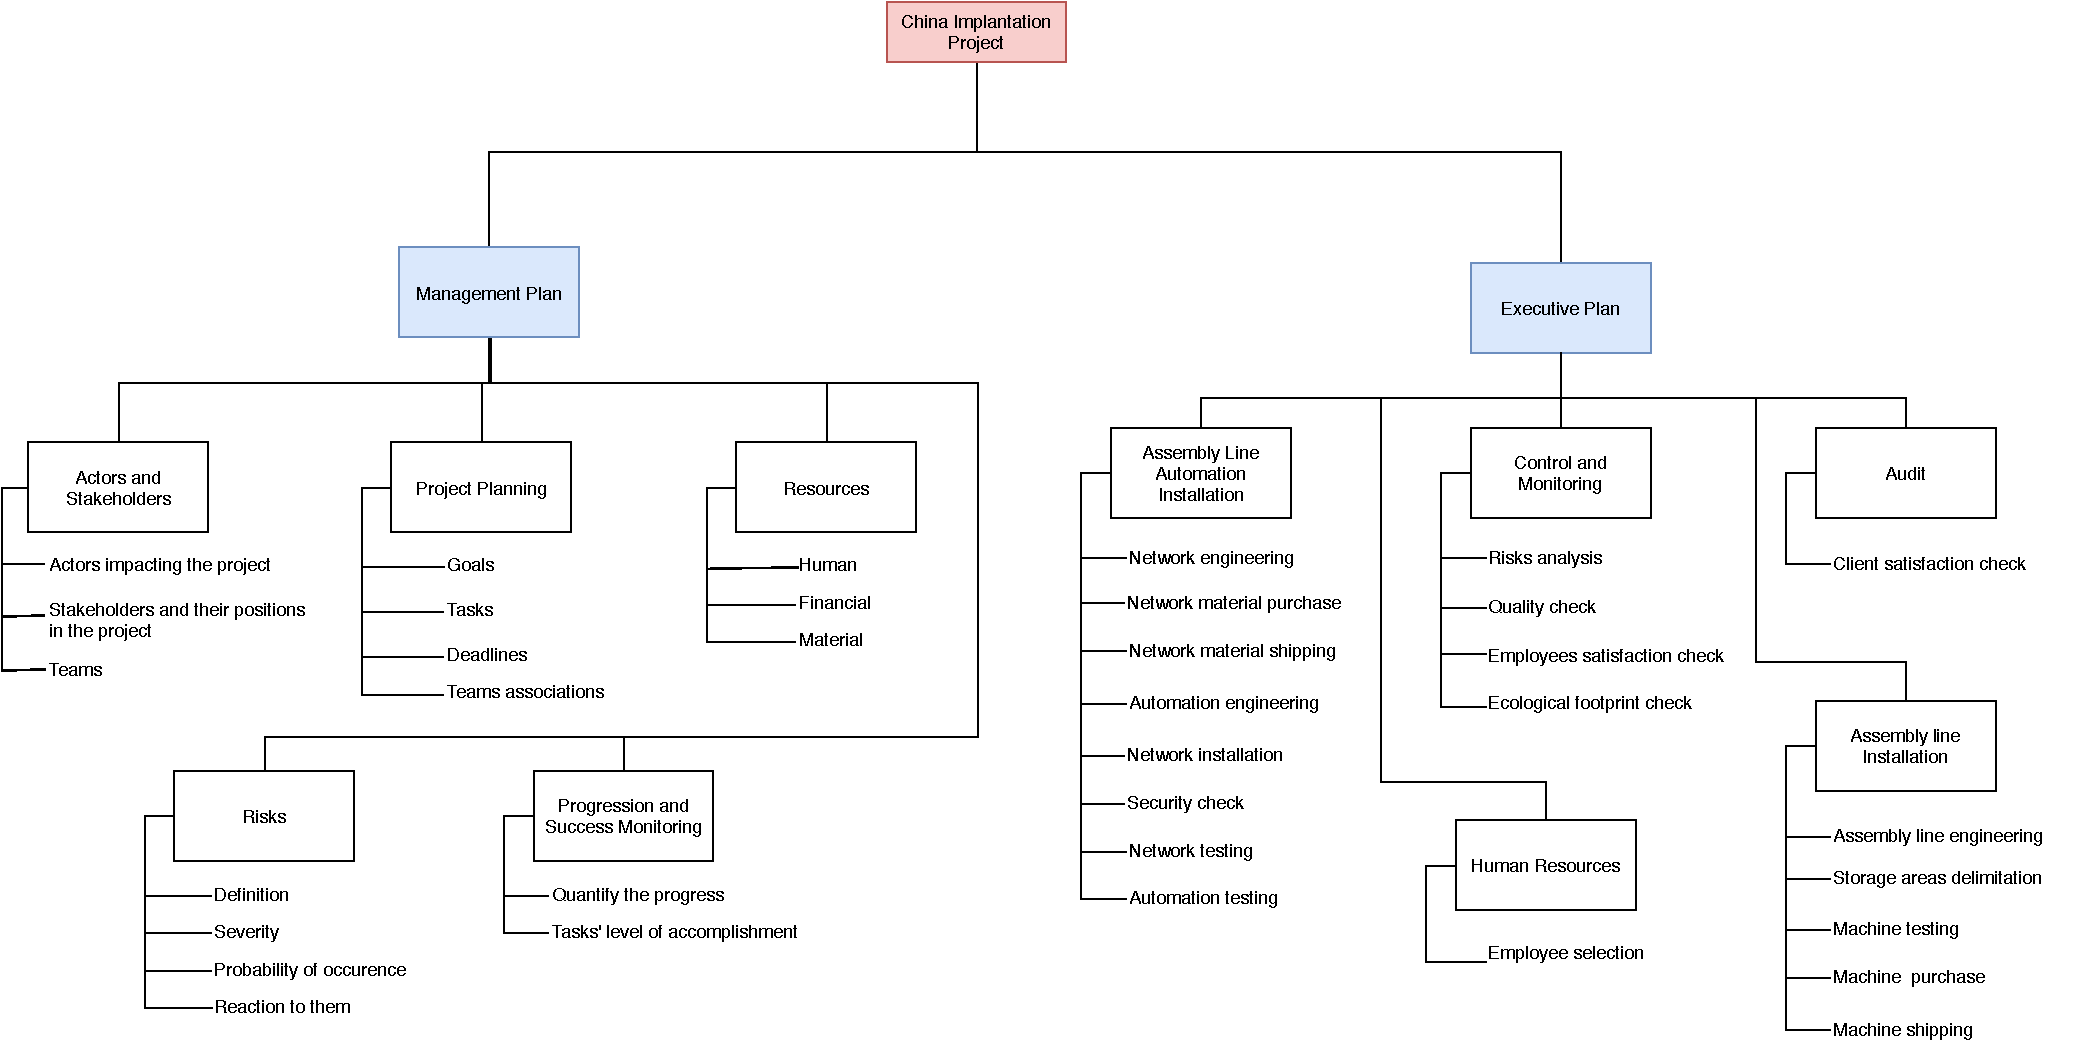
\includegraphics[scale=0.5]{Img/wbs-management-inter.pdf}
\caption{Work Breakdown Structure of the project}

\end{figure}

\subsection{Tasks}

The project is separated in many tasks that represents all steps needed to reach the goal of the project.
These tasks are separated in two categories : \emph{Managment plan} in which all the tasks represents the redaction od the management plan of the project and \emph{Executive plan} the represent the active part of the project in which the assembly line is installed.

\subsubsection{Management Plan}

The management plan is the part in which each step of the project is defined.
The management plan is defined as a frame for the project and theses tasks must be achieved before all executive task.
This part begins with a precise description of the project and goals followed by the 5 next parts.

\paragraph{Actors and Steakholders} In this parts, we must think and describe all the avtors involved in the project.
These actors are steakholders and can interact in some way with the project.
The description includes theire position, their importance and the manner that they interact with the project.
This task have also a goal of definition different teams that are required to bring this project to life.

\paragraph{Project planning} Within this task, we must think and describe all the tasks required to finish the full project, the time and resources required to achieve each task and what are task dependencies.
In this task, we must define what are deadlines and when to make debreiefing and evaluate the progression of the project.

\paragraph{Resources} In this part of the project, we must identify and write the required resources to achieve each task defined in the \emph{Project planning} part.
These resources include : human resources, financial resources and material resources.

\paragraph{Risks} In this task, we must define the primary risks that can occur during the project and how to reduce the side effect of each risk.
Each risk have a severity and prbabilty rate that represent the criticity of it.
Higher the criticity is, important the risk must be and planned with caution.

\paragraph{Progression and success monitoring} Finally, in the progression monitoring we must identify what indicator can represent the progression or the success of each task and the whole project.
These indicator will be used all along the project to define it's progression and if some task are taking late.

\subsubsection{Executive Plan}

The executive plan indicates all actions done after the work on the management plan. 
This category includes the installation of the assembly line and its automation, but also its control and monitoring, in addition of the human resources and an audit of the client.

\paragraph{Assembly Line Installation} This part aims to identify the processes brought by the installation of the assembly line. 
After an assembly line engineering, in which we study the building disposal, where and how the machines will connect with themselves, we also
study the place for the storage areas. 
We then test the machines after their purchase and their shipping. 

\paragraph{Assembly Line Automation installation} This part is about the automation of the assembly line, which includes a network engineering (the study of the disposal of the network in the building), the purchase
of the material for this network (routers, switches, etc.) and their shipping to the building, before their installation and test. 
We also study the automation of the machines, how it will work, and how to put it in place, with also a testing session and a security check.

\paragraph{Human Resources} The human resources part identify the employee selection process. Those employees 
must be fit to the required tasks of the executive plan. To the study of the building and other engineering around the machines to the 
installation of the automation of those machines, and their control and monitoring. 

\paragraph{Control and Monitoring} After the installation of the machines and their automation set, we must control and regulate them.
This includes the risks analysis process, which means a constant control and verification of the assumed risks but also an answer plan in the case of a crisis situation. 
We also check on the quality of the machines, their cleanliness and their working order, but also on the employee's satisfaction as we want to be sure they
work in an environnement as comfortable as possible. 
In the same way, we want a constant control of the ecological footprint of the building to respect our environmental engagements.   

\paragraph{Audit} Finally, this task is required to retreive some feedback from the client.
These feedback can lead to an improvement process and can be added to our quality pipeline in order to continuously improve our practices.



\section{Required resources}

% Quels sont les moyens humains nécéssaires ?
    % Equipes
    % Formations
    % Nombres d'heures
% Quels sont les moyens financiers requis ?
% Quels sont les moyens materiel requis ?

\subsection{Human cost}
The human cost we analyze represents the amount of work in days and the remuneration of everyone involved in the realization of, based on our project planning, the two parts (the initial part with the management plan, and the executive plan with the installation and monitoring of one assembly line, and the formation of the employees to the handling of the machines).
The costs are based on the total number of days of work,the persons involved, and the average price cost of the employees which you can see in this table.

\begin{figure}[h]

\centering
\includegraphics[scale=1]{Img/humanCost.png}
\caption{Average employee cost}

\end{figure}

To calculate the cost we used the working rules in France and China :
\begin{itemize}
	\item[--] In France : 35 hours of work per week and 272 days of work per year.
	\item[--] In China :  40 hours of work per week and an average of 345 days of work per year. \\
\end{itemize}

The next table will present the different type of actors (employees) of this project and how much they are paid per hour according to the average employee cost of the previous table and the working rules for each country.

\begin{figure}[h]

\centering
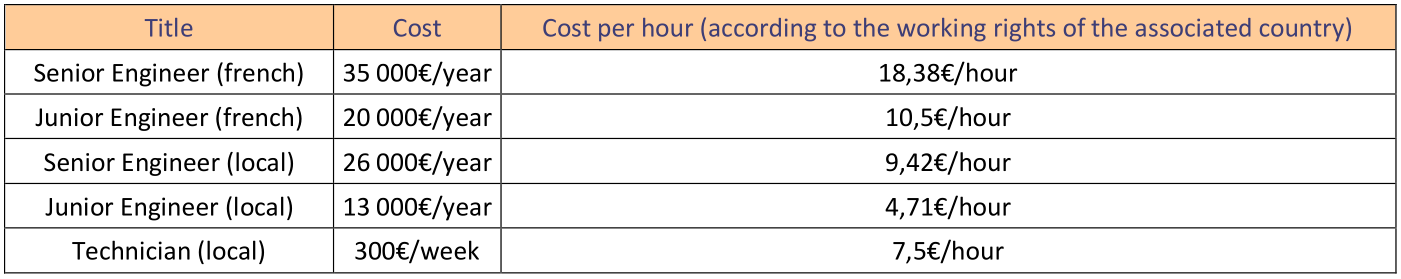
\includegraphics[scale=0.6]{Img/HumanCostPerHours.png}
\caption{Average employee costs per hour}

\end{figure}

With this data, we now analyze the number and type of the actors of each part and calculate the total cost.

\subsubsection{Initial part}
	The initial part took place during 4 days and involved a team of five french engineers, one leader senior engineer and four junior engineers.
	The cost is calculated according to the french working rule of 35 hours of work a week, so 7 hours a day.

	\begin{figure}[h]

	\centering
	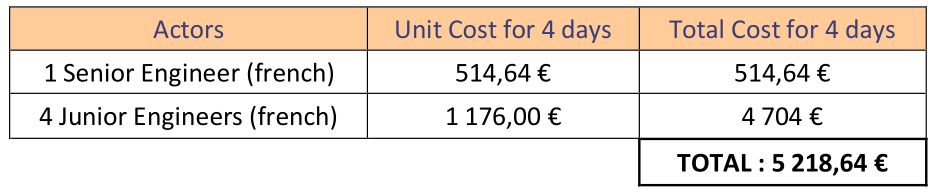
\includegraphics[scale=0.6]{Img/firstPartHumanCost.png}
	\caption{Initial part cost}

	\end{figure}

\subsubsection{Executive part}
	According to the gantt diagram, the executive part is 102 days long, minus 80 days of equipment shipping (twice 40 days), it represents 22 days of work.
	During these 22 days, 7 chinese engineers and 10 chinese technicians/regular employees (counted as technicians), as you can see here, we estimated these numbers while partitionning the executive part (installation and monitoring/control) in different tasks. \\

	\begin{figure}[h]

	\centering
	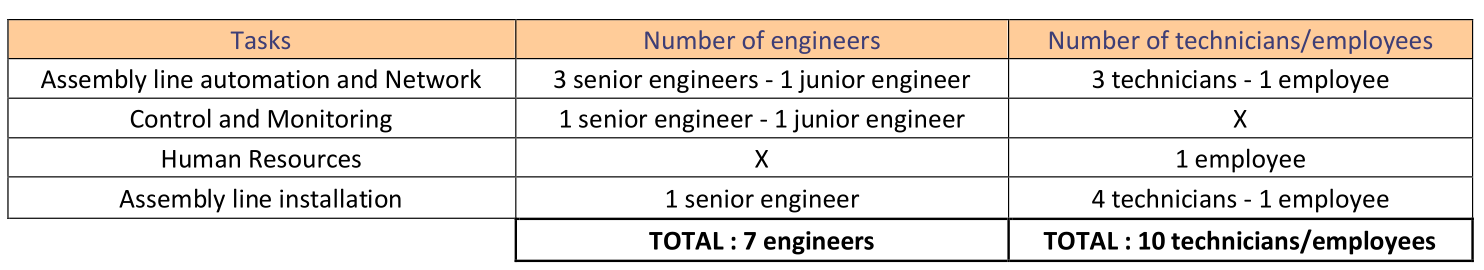
\includegraphics[scale=0.6]{Img/secondPartNbrHuman.png}
	\caption{Number of employees for the executive part}

	\end{figure}

	The cost is calculated according to the chinese working rule of an average of 40 hours of work a week, so 8 hours a day.

	\begin{figure}[h]

	\centering
	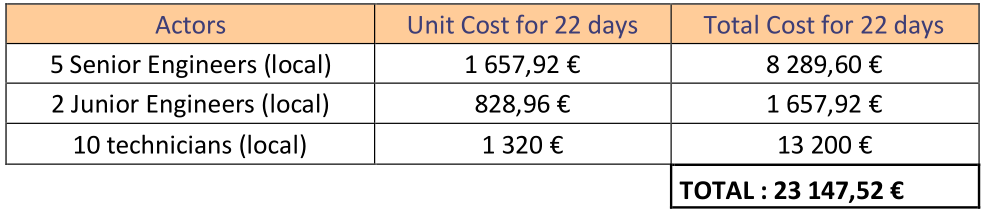
\includegraphics[scale=0.6]{Img/secondPartHumanCost.png}
	\caption{Executive part cost}

	\end{figure}

\subsubsection{Formation}
	The 17 employees involved in the executive part need to be tought how an assembly line works, how to handle the machines, how they work and also their security rules. 

	We estimated the cost of such a formation of 3000 euros per person (a total of 51 000 euros for the 17 employees) and 5 days, also counted as 5 days of works for them.

	\begin{figure}[h]

	\centering
	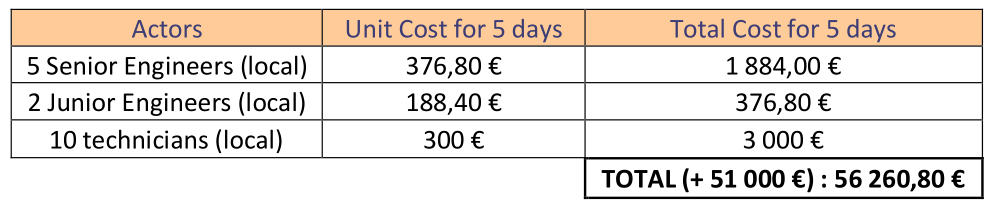
\includegraphics[scale=0.6]{Img/formationCost.png}
	\caption{Formation cost}

	\end{figure}

With these three parts, we reach a total human cost of \textbf{84 626.96 euros.} \\

\subsection{Material cost}
This cost is about every material directly used in one assembly line and its cost.
Our assembly line will include : \\
\begin{itemize}
	\item[--] Handle molds, to make the brush handle (an average of 2 per injection machine).
	\item[--] An injection machine, to mold the shape of the toothbrushes.
	\item[--] A tufting machin to tuft on brush holders.
	\item[--] A trimming and end rounding machine to cut and shape the bristles to the manufacturers specification, and to round them to be softer and more comfortable to the teeth.
	\item[--] A fully automated packaging machine to pack the toothbrushes.
	\item[--] And of course conveyers belt which will link these machines together. We estimated an average of 4 meters between machines, so we would need around 16 meters of it. \\
\end{itemize}

All of it would be around 30 square meters. \\
We have access to two types of injection machines, a 50T and a 80T, which means it is a 50/80 ton servo-motor operated machine, the maximum clamping force with these machines is either 50 or 80 tons. Servo-motors are used for energy saving, so these machines give the highest energy saving in hydraulic machines. In this estimation we chose the 80T injection machine for a better energy saving.

To calculate the total cost, we used this table of average prices. \clearpage

\begin{figure}[h]

	\centering
	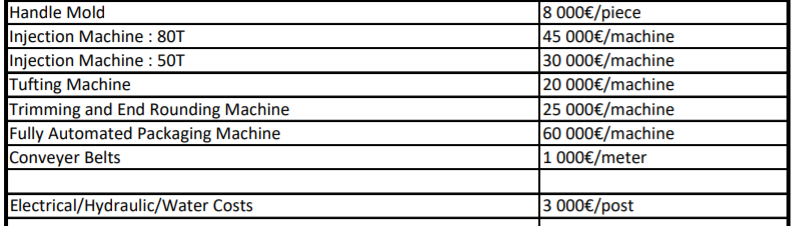
\includegraphics[scale=0.9]{Img/averageMachineCost.png}
	\caption{Average machine costs}

\end{figure}

We have 5 machines in our assembly line. We decided, for the electrical/hydraulic/water costs, that there will be a maximum of 3 machines by post, so 2 posts for one assembly line, which will cost 6 000 euros.

\begin{figure}[h]

	\centering
	\includegraphics[scale=0.6]{Img/machineCost.png}
	\caption{Machines costs for one assembly line}

\end{figure}

So, the total machine cost for one assembly line is \textbf{188 000 euros}.

We reach a total estimation cost of \textbf{272 626.96 euros} with both the human cost and the machine cost.


\section{Risks management plan}
\label{risk-management}
Considering that Mold \& Co's new production plant implies an important
and complex system, we have to identify and evaluate all the risks
inherent to this system in order to limit them the most possible. This
risk analysis will allow us to help designing the new production system
by establishing the most efficient preventive and correctives measures.

In order to deal with the risk management, we decided to use the FMECA
Method on the means of production of Mold \& Co company. This means that
we consider all the risks related to the operation of the assembly line
system.

\subsection{Plan}

For that purpose, we have to, as a first step, describe the overall
production system. Then we will be able to identify all the threats.
After this step, we will identify all the threats that could affects the
system and assess them in order to define their criticality.

Ultimately, we will see how to compensate these eventual failure modes
where appropriate.

\subsection{Description of the system}

The assembly line system is composed of two main parts : the mechanical
system and the computing's one.

By the way, we estimate that these two systems are interdependent. In
other words, we have to take into account that if the mechanical part of
the assembly line fails, the entire system cannot work anymore and vice
versa.

Actually, mechanical part of the production chain can work independently
but if the computing system is not working, the mechanical will
encounter problems about its regulation and monitoring.

\subsection{Definition of the risk assessment}

According to the FMECA Method, we have to assess three different values
in the table of risk.

First of all, the Severity (S) which equals to the importance of the
consequences that the risk could induce on the production of the
factory. More the risk can affect the production line, more the Severity
level is high as the following table shows :

\begin{figure}[h]
    \centering
    \begin{tabular}{| p{4cm} | c | c |}
        \hline
        \rowcolor{heading-color}\multicolumn{1}{|c|}{Severity definition} & Severity level & Associated color\\
        \hline
        Insignificant & 1 & green  \\
        \hline
        Minor & 2 & light green  \\
        \hline
        Significant & 3 & yellow  \\
        \hline
        Serious & 4 & orange  \\
        \hline
        Major & 5 & red  \\
        \hline
    \end{tabular}
    \caption{Table of severity level}
\end{figure}

    Regarding the Occurrence (O), it enables to measure the likelihood of the risk. Mire the risk is potential, more the Occurrence value is high as we can see as below :

    \begin{figure}[h]
        \centering
        \begin{tabular}{| p{4cm} | c | c |}
            \hline
            \rowcolor{heading-color}\multicolumn{1}{|c|}{Occurrence definition} & Occurrence level & Associated color\\
            \hline
            Remote & 1 & green  \\
            \hline
            Very low & 2 & light green  \\
            \hline
            Low & 3 & yellow  \\
            \hline
            Moderate & 4 & orange  \\
            \hline
            Major & 5 & red  \\
            \hline
        \end{tabular}
        \caption{Table of occurence level}
\end{figure}

Finally, the Detection (D) is measured according to the ease for the operators to discover a failure mode. Higher the value is, easier it is to detect the failure.

\begin{figure}[h]
    \centering
    \begin{tabular}{| p{4cm} | c |}
        \hline
        \rowcolor{heading-color}\multicolumn{1}{|c|}{Detection definition} & Detection level\\
        \hline
        Blatant & 1  \\
        \hline
        Easily identifiable & 2  \\
        \hline
        Discreet & 3  \\
        \hline
        Hard to identify & 4 \\
        \hline
        Very  hard to identify & 5 \\
        \hline
    \end{tabular}
    \caption{Table of detection level}
\end{figure}

Severity, Occurrence and Detection are arbitrarily assessed whereas Criticality and RPN are calculated from these same data.\\

Especially, we have the following relations :
\begin{itemize}
    \item Criticality = Severity \* Occurrence
    \item RPN = Severity \* Occurrence \* Detection = Criticality \* Detection
\end{itemize}

These last two measures enable us to prioritize the risk in order to make the further effort in order to limit them and eventually resolve them if ever they occur.

\section{Calculation of the criticality and risk priority numbers}

In sum, Severity, Occurrence and Detection are arbitrarily assessed
whereas Criticality and RPN (Risk Priority Number) are calculated from these same data.

Especially, we have the following relations :

\[Criticality = Severity \times Occurrence\]
\[RPN = Severity \times Occurrence \times Detection = Criticality \times Detection\]

These last two measures enable us to prioritize the risk in order to
make the further effort in order to limit them and eventually resolve
them if ever they occur.

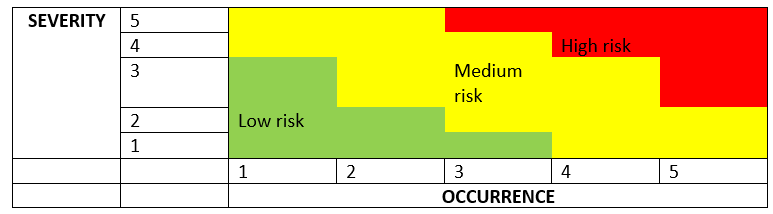
\includegraphics{Img/img-risk.png}

After having defined all the measure required in order to assess the risks. We can now list them,  

evaluate their Severity (S), Occurrence (O), Detection (D) and thus calculate for each one, their criticality (C) and their Risk Priority Number (RPN). 

\begin{landscape}
\begin{figure}[h]
\centering
\resizebox{\textwidth}{!}{%
\begin{tabular}{|l|p{3cm}|p{3cm}|p{3cm}|p{3cm}|p{3cm}|l|l|l|l|l|}
\hline
Identifier & Failure mode               & Failure causes                     & Failure effect                      & Detection method                  & Corrective actions                                & S & O & D & C  & RPN \\
\hline
A          & Power outage               & Equipment disfunction              & Stop of the production              & Beep                              & Inverter and external batteries                   & 5 & 4 & 1 & 20 & 20  \\
\hline
B          & Noise pollution            & Equipment disruption               & Employee’s discomfort               & Error message                     & Automatic measurement and earplugs                & 1 & 2 & 2 & 2  & 4   \\
\hline
C          & Inherent materiel defect   & Obsolescence                       & Slowdown or stop of the production  & Error message                     & Periodic maintenance                              & 5 & 4 & 2 & 20 & 40  \\
\hline
D          & Earthquake                 & Environment                        & Stop of the production              & Sound and tremors                 & Earthquake protection                             & 4 & 1 & 1 & 4  & 4   \\
\hline
E          & Fire                       & Overheat                           & Stop of the production              & Beep (fire alarm), flames         & Fire prevention system                            & 4 & 1 & 1 & 4  & 4   \\
\hline
F          & Lack of raw materials      & Desynchronization                  & Stop of the production              & Alert message                     & Provider proximity and Daily stock’s review       & 4 & 2 & 1 & 8  & 8   \\
\hline
G          & Short circuit              & Equipment disfunction              & Slowdown or stop of the production  & Alert message                     & Circuit-breakers                                  & 4 & 3 & 1 & 12 & 12  \\
\hline
H          & Absence of a main operator & Leave                              & Relative stop of the production     & Control presence of the employees & Control presence of the employees                 & 3 & 4 & 1 & 12 & 12  \\
\hline
I          & Local network outage       & Broken cable                       & Stop of the production              & Error message                     & Network connection cable redundancy               & 5 & 5 & 1 & 25 & 25  \\
\hline
J          & Lightning                  & Environment                        & None                                & Lightning sound                   & Lightning rod                                     & 1 & 1 & 1 & 1  & 1   \\
\hline
K          & Flood                      & Water leak                         & Eventual stop of the production     & Leak detectors                    & Water recycling system                            & 2 & 3 & 1 & 6  & 6   \\
\hline
L          & Over-voltage               & Insulation failure                 & Stop of the production              & Alert message                     & Circuit-breakers                                  & 4 & 2 & 1 & 8  & 8   \\
\hline
M          & Vandalism                  & Human error                        & Slowdown or stop of the production  & Cameras                           & Cameras and Intern investigation                  & 4 & 2 & 2 & 8  & 16  \\
\hline
N          & Overload                   & Equipment dysfunction (disruption) & Slowdown or stop of the production  & Error message                     & Regular control of the equipment’s settings       & 4 & 3 & 2 & 12 & 24  \\
\hline
O          & Product quality defect     & Human error                        & Slowdown of the production          & Block of the equipment            & Regular quality controls                          & 2 & 3 & 1 & 6  & 6   \\
\hline
P          & Environmental pollution    & Equipment dysfunction (disruption) & Penalty                             & Pollution traces                  & Regular analysis on the water and other resources & 3 & 3 & 3 & 9  & 27  \\
\hline
Q          & Non respect of deadlines   & Wrong estimation of the delays     & Economic losses                     & Project management                & Recursive estimation                              & 3 & 5 & 2 & 15 & 30  \\
\hline
R          & Employee’s injury          & Accident                           & Eventual slowdown of the production & Complain                          & None                                              & 3 & 1 & 1 & 3  & 3  \\
\hline
\end{tabular}%
}
\caption{Risk table}
\end{figure}
\end{landscape}

\begin{figure}[h]
    \centering
    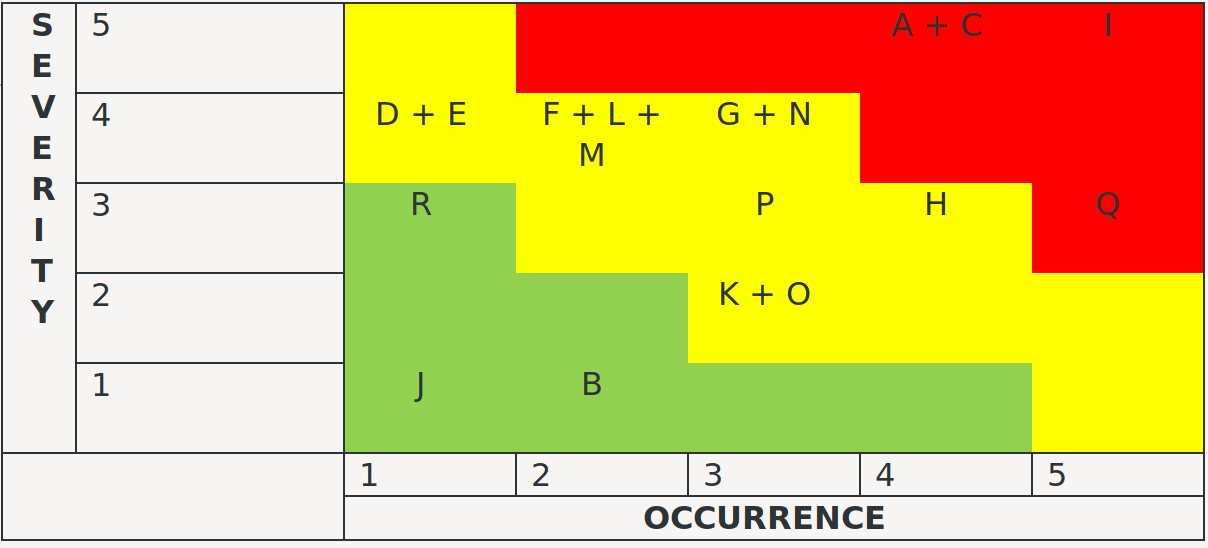
\includegraphics[scale=0.3]{Img/severity.png}
    \caption{Table of severity}
\end{figure}

\subsection{Prevention and correction of the risks}

What we can conclude from this table is that four risks : A, C, I and Q
are particularly important as their criticality is in the red color so
high priority.

Then we have to pay a special attention to these one and foresee strong
corrective actions in order not only for prevention but also for
correction.

Particularly, for these risk we decided to :

\begin{itemize}
\item
  Power outage (A) : provide external batteries while the failure is not
  resolved
\item
  Inherent materiel defect (C) : plan periodic maintenance on all the
  different machine consisting in verifying all its functionalities
\item
  Local network outage (I) : foresee a double connection on the machines
  for the local network so that if one is defaulting, the other will
  relay the connection
\item
  Non respect of the deadlines (Q) :

  \begin{itemize}
  \item
    foresee provisional timeline of 10\% of the time required to achieve
    the project
  \item
    daily checks of the projects progress
  \end{itemize}
\end{itemize}

% Quels sont les risques encourus durant le projet ?
% Quel est la sévérité, la probabilité d'apparition ?
% Quel opérations mettre en place pour les risques les plus graves ?

\section{Indicators of progression and success}

Il est important de mesurer de façon continue l'évolution du projet. C'est pour cela que la section qui va suivre traitera des indicateurs clés de performance.

La représentation de tous les indicateurs choisis sont inscrits dans un tableau où l'on retrouve : 
\begin{itemize}
    \item le nom de chaque indicateur,
    \item l'objectif défini au début du projet,
    \item la valeur réelle de l'indicateur.
\end{itemize}

Si l'indicateur est a vert, il faudra poursuivre les actions en cours afin de maintenir ce bon résultat.
Si l'indicateur est au rouge, vous devez prendre les mesures correctives nécessaires.
Si l'indicateur est au orange, il faut alors le surveiller.

Les indicateurs clés de performance sont à suivres de près, en effet, ils ont d'une certaine façon, un impact financier sur le projet. Si l'indicateur est au rouge, les mesures correctives qui s'imposent généreront des dépenses additionnelles. Toutefois, si l'indicateur est au vert, c'est que tout se déroule comme prévu.

Nous classerons nos indicateurs clés de performance sous quatre catégoris : 
\begin{description}
    \item[Les délais]: le projet se déroule dans les temps
    \item[Le budget]: budget dépassé ? 
    \item[La qualité] : la progression du projet est-elle satisfaisante ?
    \item[L'efficacité] : Le projet est-il gérer de manière efficace ?
\end{description}

% Comment peut on quantifier l'avancement du projet ?
% Quel est l'indicateur permettant de définir qu'une tache est accomplie et valide ?

\section{Conclusion} 



\end{document}

